

\documentclass[10pt]{sensys-proc}
\usepackage{graphicx}
\usepackage{balance}
\usepackage{comment}
\newcommand{\redcolor}[1]{\textcolor{red}{#1}}

\newcommand{\figref}[1]{Figure~\ref{#1}}
\newcommand{\secref}[1]{Section~\ref{#1}}
\newcommand{\tabref}[1]{Table~\ref{#1}}
\newcommand{\algoref}[1]{Algorithm~\ref{#1}}
\usepackage{graphicx}
\usepackage{subfig}
\usepackage{blindtext}
\usepackage{array}
\usepackage{caption}
\usepackage{url}
\usepackage{epstopdf}
\usepackage{multirow}
\usepackage{xcolor,colortbl}

\newcommand{\pushline}{\Indp}
\definecolor{Gray}{gray}{0.91}
\newcolumntype{a}{>{\columncolor{Gray}}c}

\numberofauthors{2}

\author{
%
% The command \alignauthor (no curly braces needed) should
% precede each author name, affiliation/snail-mail address and
% e-mail address. Additionally, tag each line of
% affiliation/address with \affaddr, and tag the
%% e-mail address with \email.
\alignauthor Alice Security \\
        \affaddr{Department of Computer Science}\\
        \affaddr{University of Southern California}\\
       \email{alice@example.edu}
\alignauthor Bob Privacy \\
    \affaddr{Networked Embedded Systems Group}\\
    \affaddr{Swedish Institute of Computer Science}\\
    \email{bob@example.se}
}

\title{Buildsys}

\crdata{978-1-4503-1169-4}
\conferenceinfo{SenSys'13,} {November 11--15, 2013, Rome, Italy.}
\CopyrightYear{2013}

\begin{document}

\maketitle

\begin{abstract}
This paper provides a sample of a \LaTeX\ document for ACM Sensys. 
It complements the document \textit{Author's (Alternate) Guide to
Preparing ACM SIG Proceedings Using \LaTeX$2_\epsilon$\ and Bib\TeX}.
This source file has been written with the intention of being
compiled under \LaTeX$2_\epsilon$\ and BibTeX.

To make best use of this sample document, run it through \texttt{pdflatex}
and \texttt{bibtex} to directly produce a pdf document.
\end{abstract}

% A category with the (minimum) three required fields
\category{H.4}{Information Systems Applications}{Miscellaneous}
%A category including the fourth, optional field follows...
\category{D.2.8}{Software Engineering}{Metrics}[complexity measures, performance measures]

\terms{Delphi theory}

\keywords{ACM proceedings, \LaTeX, text tagging}

\section{Introduction+Related Work}
  \label{sec:intro}

\begin{itemize}
\item Why buildings must be targeted for energy \cite{evans09}
\item Importance of feedback \cite{darby}
\item Why we need deployments
\item Previous such residential deployments, some of which were presented in Buildsys itself \cite{hitchhiker_residential,hitchhiker_wsn,scale_wsn}
\item Some applications-NILM\cite{hart,survey1}, Fixture Finder \cite{fixturefinder}
\item Specific learnings from our deployment, some of them complement the ones given earlier \cite{hitchhiker_residential}
\begin{itemize}
\item Glowing LED in night
\item Deployments should be transparent
\item Noisy server owing to dust (specific to developing countries)
\item Electricity failure- as a consequence all systems should be capable to restart upon resumption of electricity
\item Unreliable internet -Forcing to use Sense-Store-Upload paradigm
\item Normalization -Voltage fluctuation, different measurement by different instruments

\end{itemize}
\end{itemize}

\section{Deployment}
In this section we describe about our deployment. \figref{fig:overall} shows overall home deployment.
Following computation resources (SBC/Servers were used)
\begin{itemize}
\item X RPi
\item Plug Computers
\item Main server
\end{itemize}
Following sensors were used.
\begin{itemize}
\item EM6400 smart meter: We used pyModbus to sample at 1 Hz. Gives 40 parameters including reactive power. Reactive power can greatly help in improving NILM accuracy \cite{hart}. 
\item Appliance level meters: jPlug and Current Cost. jPlug gives data at 1 Hz and gives 10 parameters including reactive power. Current cost was needed for one appliance- electric motor.
\item CT monitoring: Custom hardware based on  XYZ.
\item Multisensors: Measure motion (based on polling), light and temperature
\item Water meter: 10 litre events. 
\item Android phones measuring x, y, z using FunF Journal\footnote{\url{http://www.funf.org/journal.html}}
\end{itemize}
Apart from this following soft-sensor streams were collected.
\begin{itemize}
\item Network statistics
\item CPU, Memory usage for all computing resources. This was to serve as preventive measure.
\item Weather streams
\end{itemize}
\begin{figure*}     
    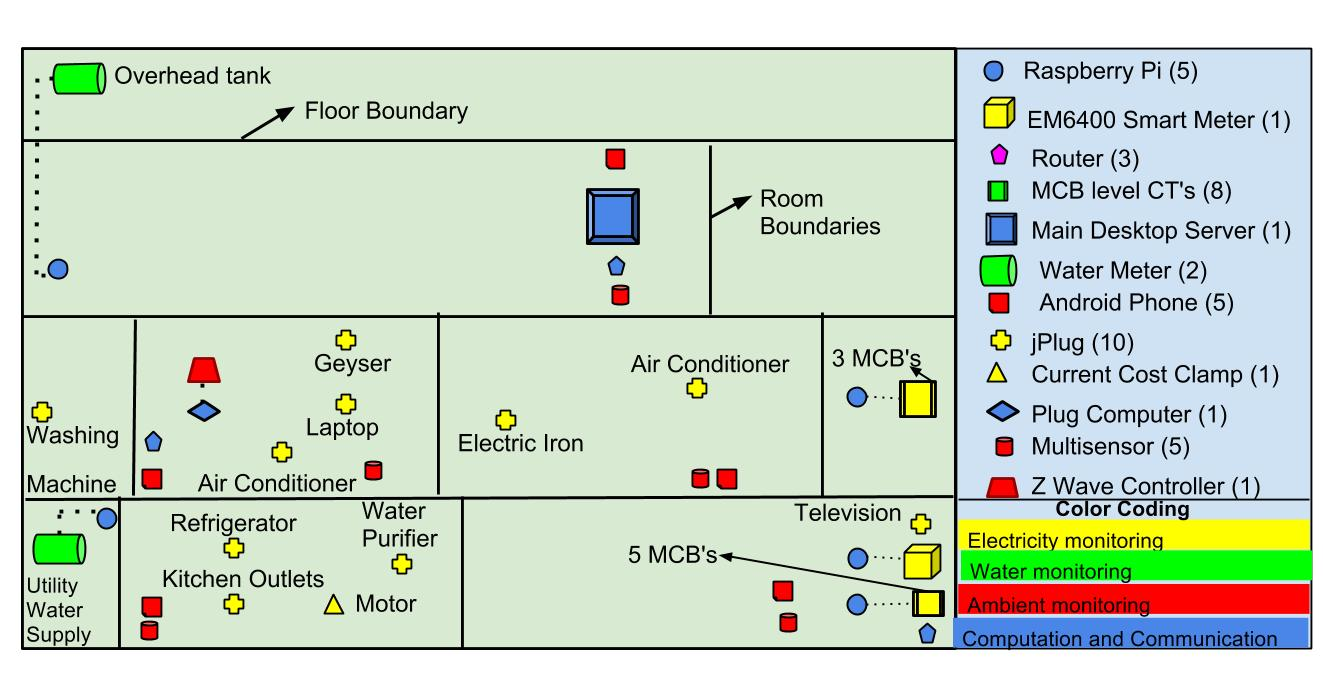
\includegraphics[scale=0.4]{./figures/overall_deployment.jpg}    
    \caption{Schematic showing overall home deployment}   
    \label{fig:overall}
   
\end{figure*}


\begin{figure*} 
    
    \subfloat[\scriptsize EM6400 Smart Meter]{
    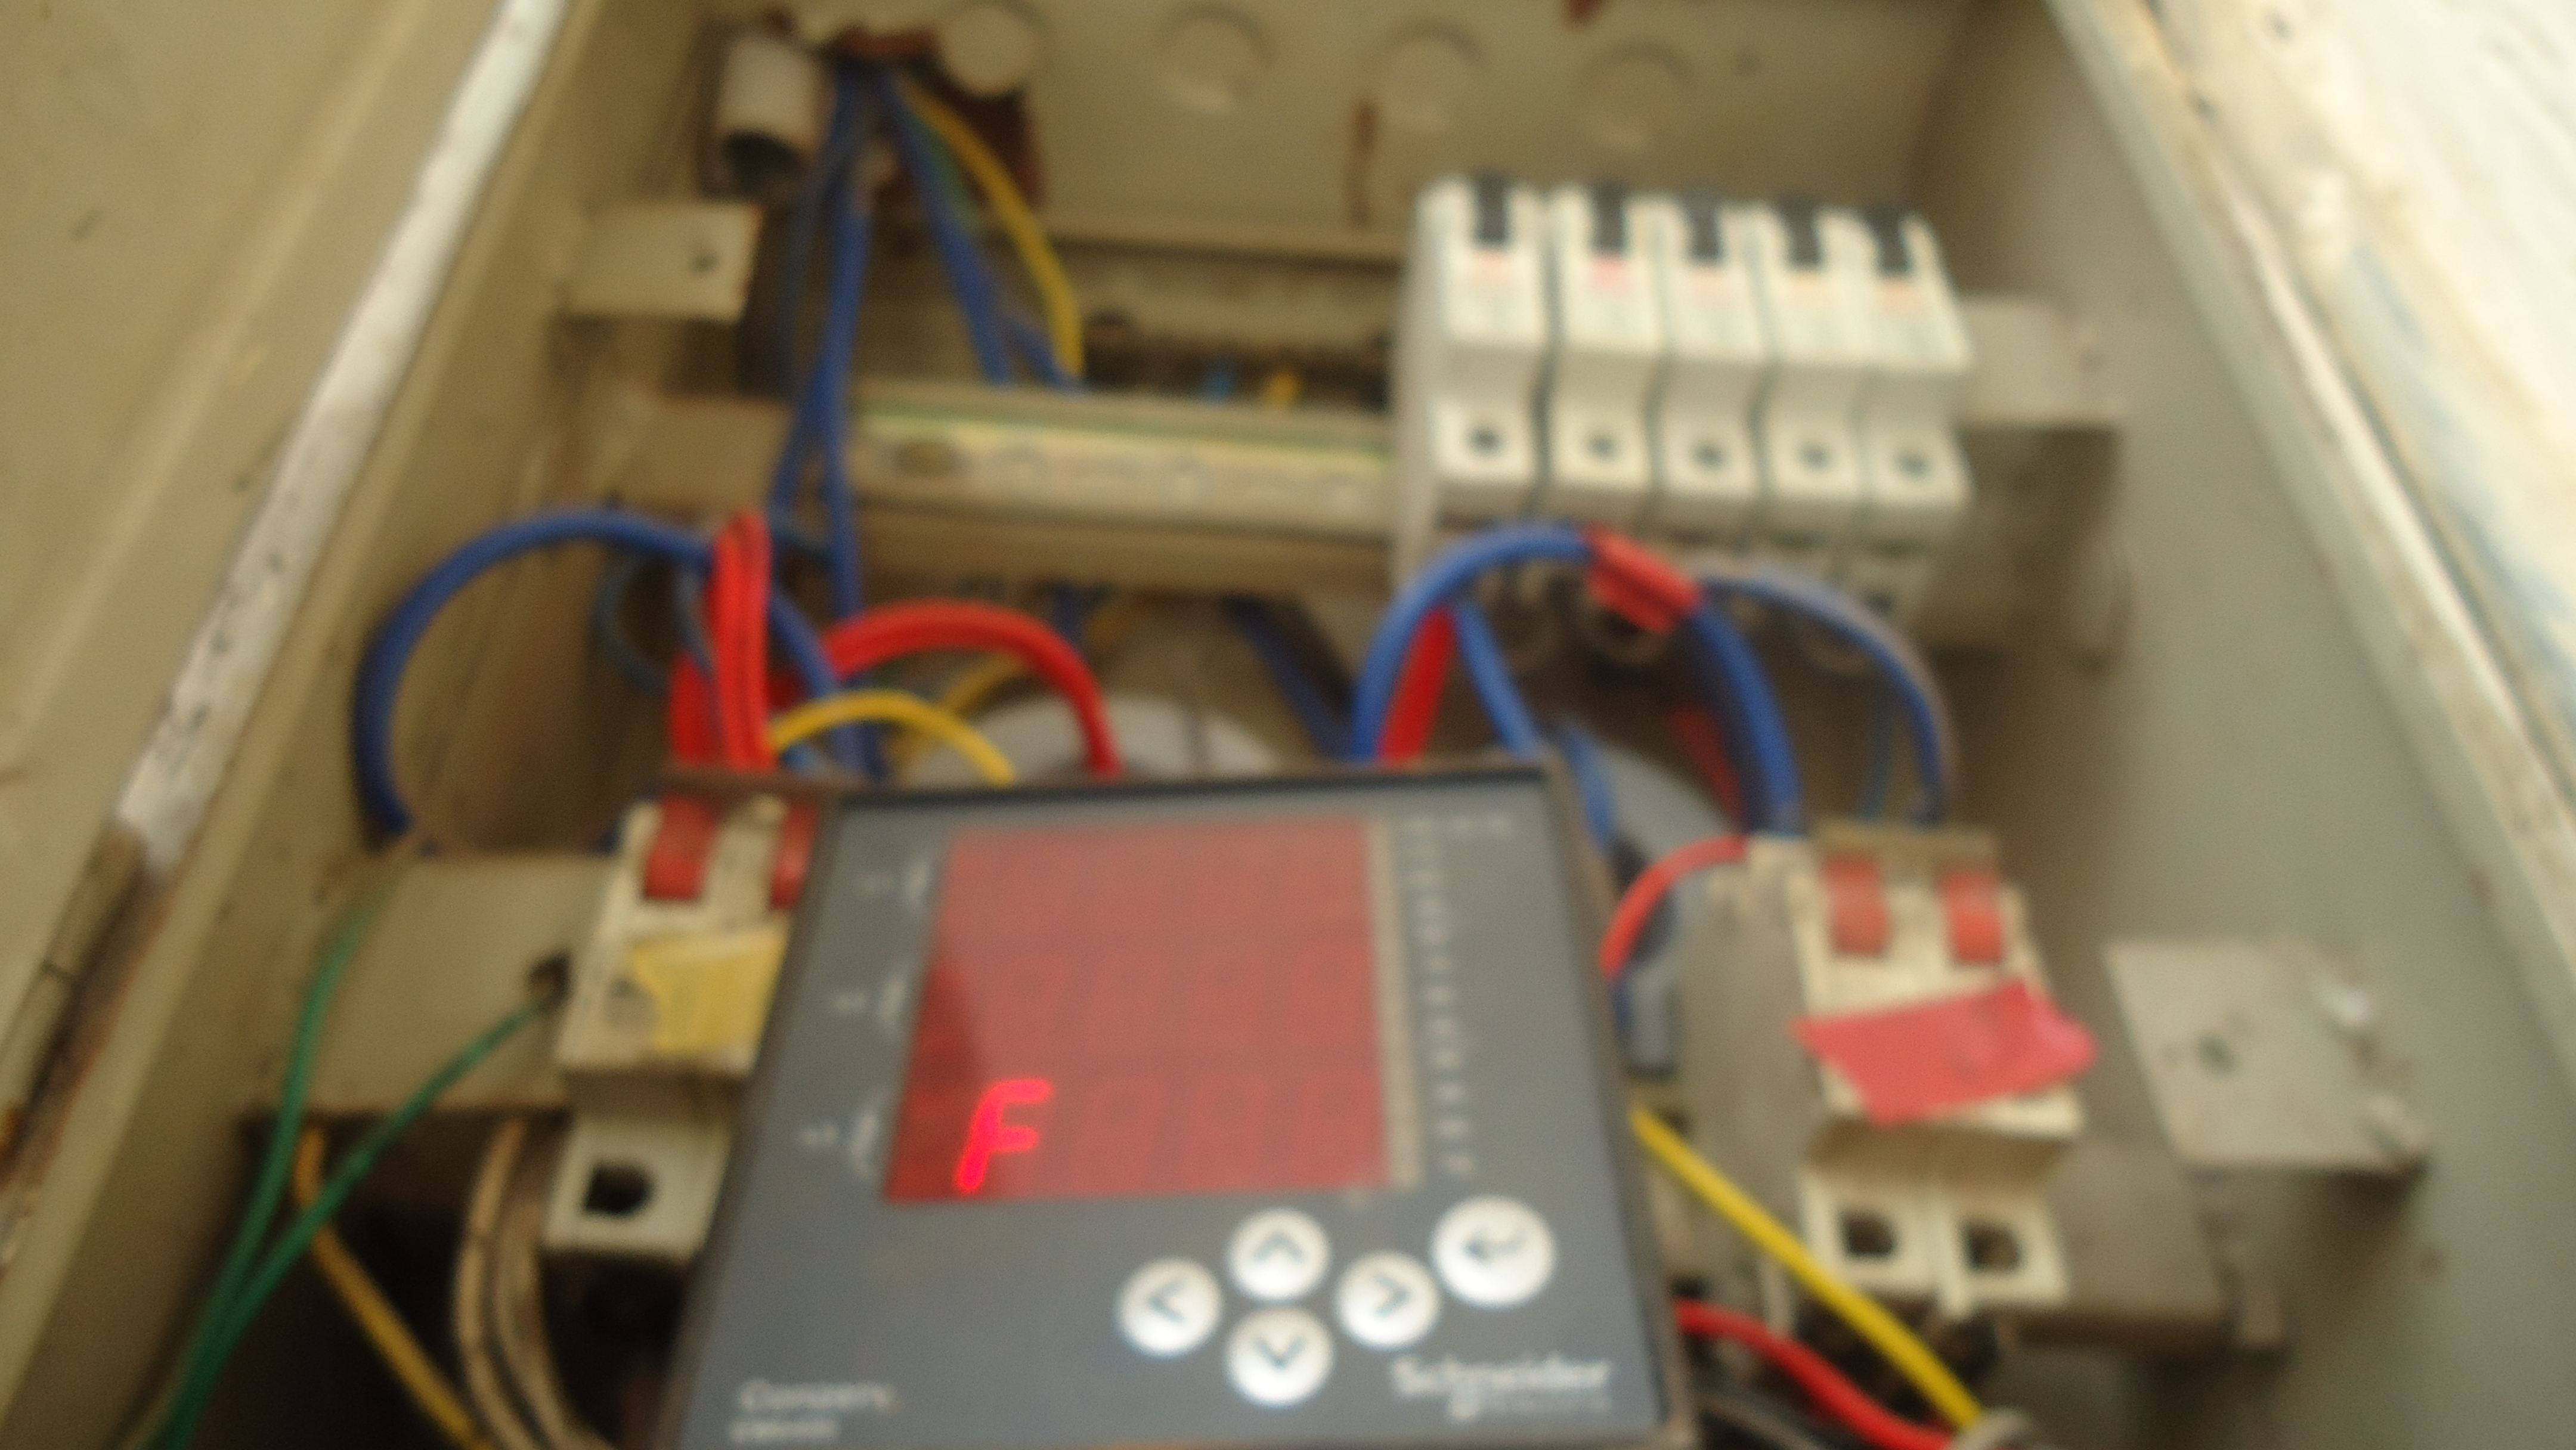
\includegraphics[scale=0.04]{./figures/electric_meter.JPG}}
    %\hspace{0.02\columnwidth}
    \subfloat[\scriptsize Water Meter]{
        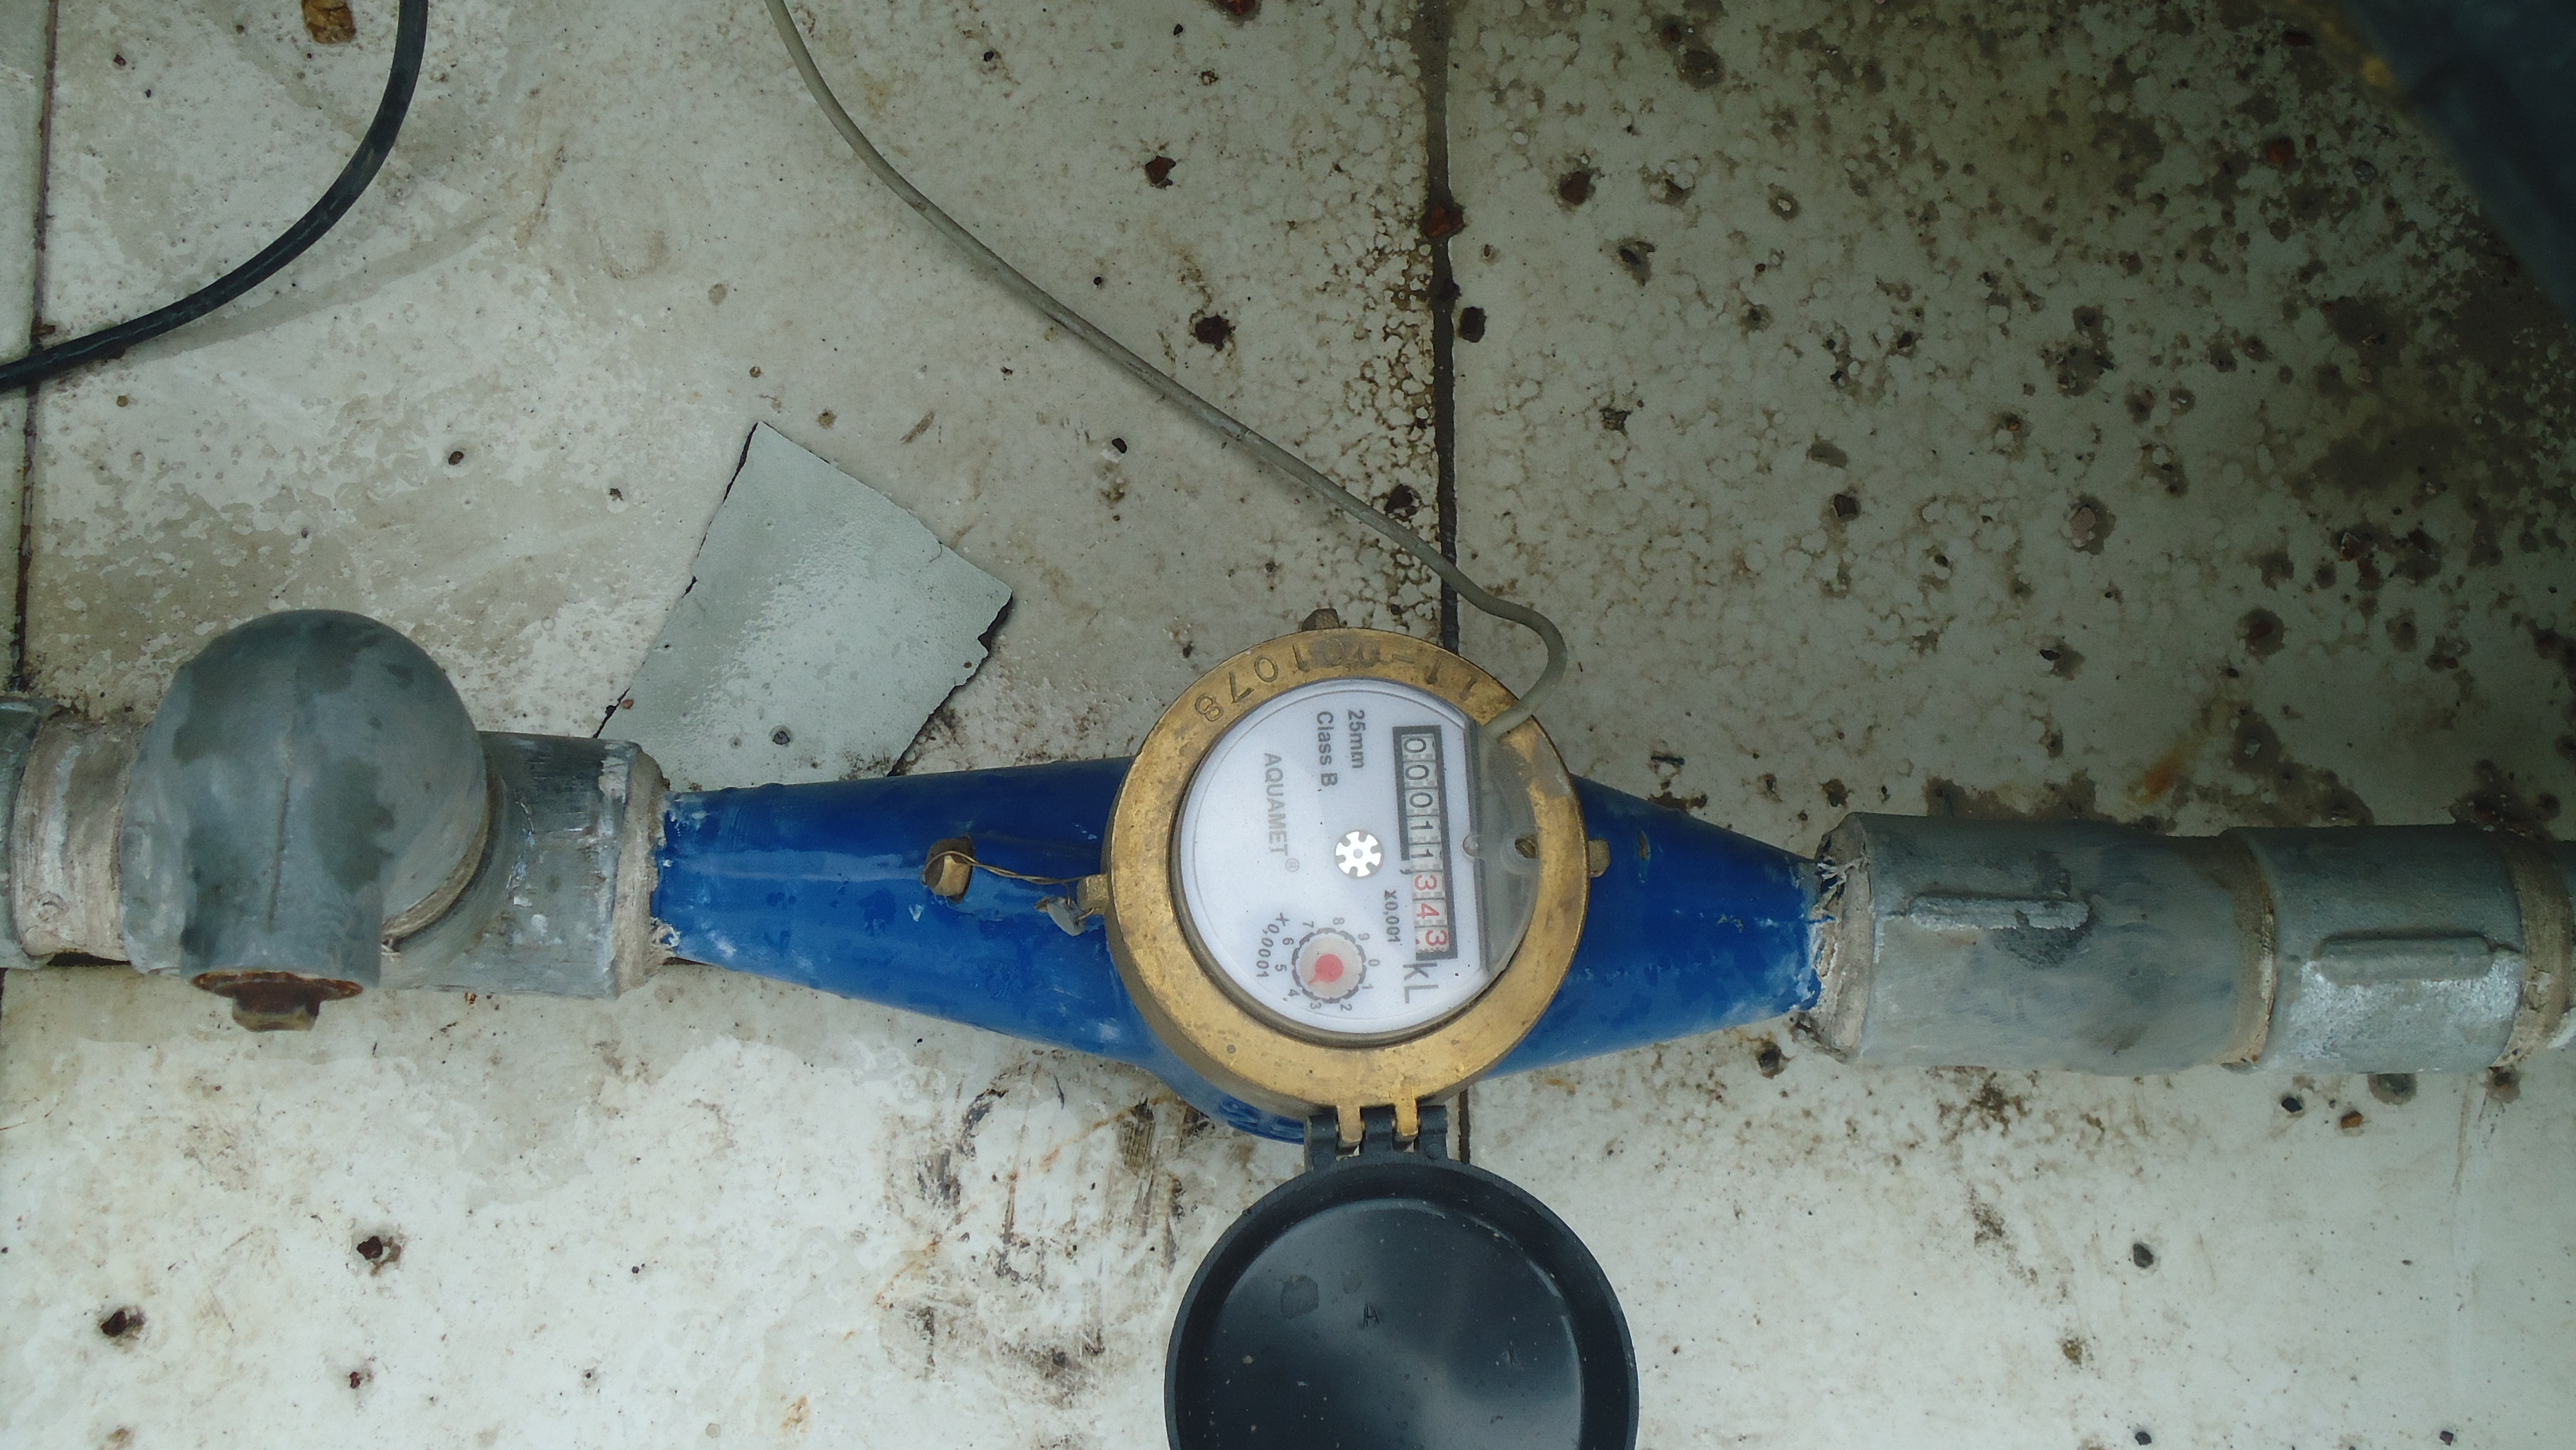
\includegraphics[scale=0.04]{./figures/water_meter.JPG}}

    \caption{Deployment Pictures}

    \label{fig:deployment}

\end{figure*}

\section{Learning}
In this section we discuss the learning from previous work in similar domains and present unique aspects which came up in our deployment.
\begin{itemize}

\item Homes are not power panacea. We have a very special case of electricity failure. Add figure
for electricity number of hours failure, failure by n'th hour, hist of failure hours
\item Homes have poor connectivity. This forced us to develop a different paradigm which we call Sense-Store-Transfer. This is shown in \figref{fig:network}

\item Homes are hazardous environments
\begin{itemize}
\item Multi failed when put on inverter point
\item Node in one room will always fail
\item Wire snag and how it led to data loss of node 4
\end{itemize}

\item Homes are remote environments:
We had to raise ~60 new issues on Github. We first did deployment in researchers home which had full access to all nodes.
We also provided alerting mechanisms.

\item User participation
Even at researchers home, had asked the researcher to take notes. But even his engagement was not 100 \%.

\item Aesthetics matter
\begin{itemize}
\item LED in night
\item Noise- Noisy SMPS due to dust. Unique to our setting. Figure from FunF showing sound level before and after cleaning.
\end{itemize}

\item Simplify the architecture
We used Load-Store-Forward. Describe this in more detail and relate to earlier n/w connectivity.
Also when number of systems is so large, simple CSV uploading is the best mechanism.

Wherever possible use Ethernet with repeaters. Also, RPi are known to have problems with WiFi.

\item Importance of meta data and calibration
Figure showing power consumption of ref. after repair
Figure showing different measurements for same appliance
Figure showing voltage fluctuations


\end{itemize}
\begin{figure}     
    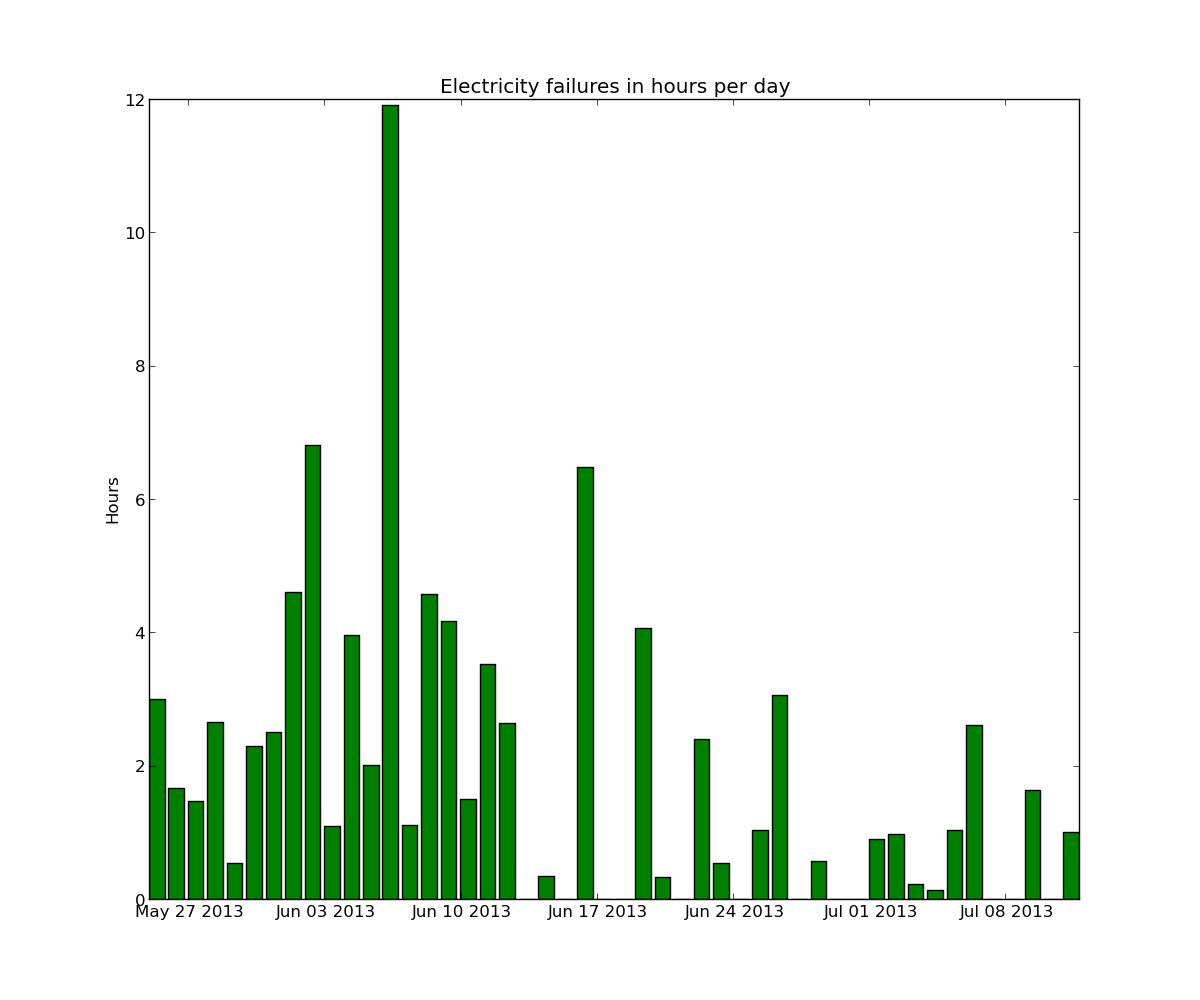
\includegraphics[scale=0.30]{./figures/electricity.png}    
    \caption{Electricity failure in hours}   
    \label{fig:failure_hours}   
\end{figure}

\begin{figure}     
    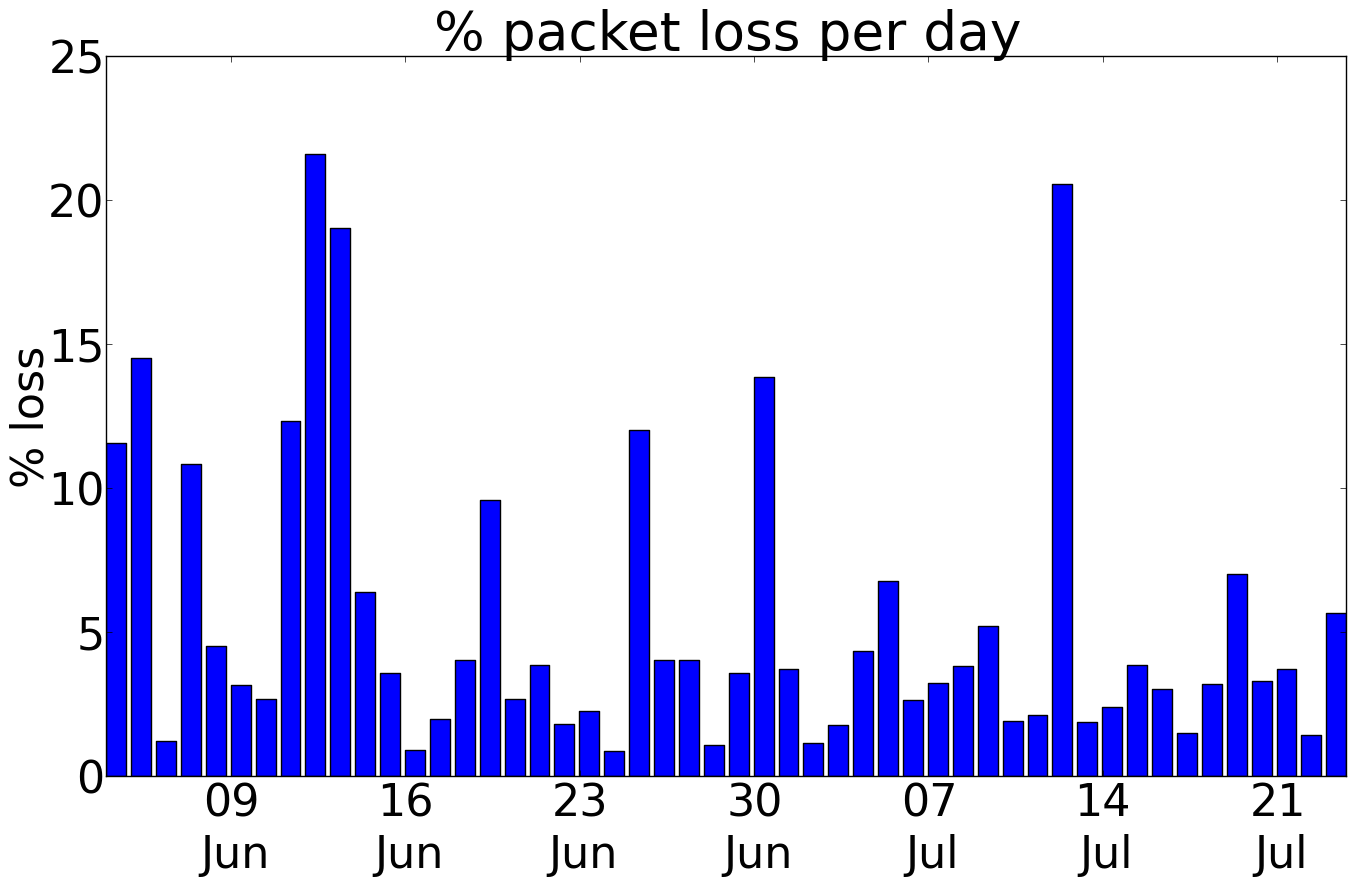
\includegraphics[scale=0.30]{./figures/network.png}    
    \caption{Overall packet drop while accessing internet}   
    \label{fig:network}   
\end{figure}

\begin{figure}     
    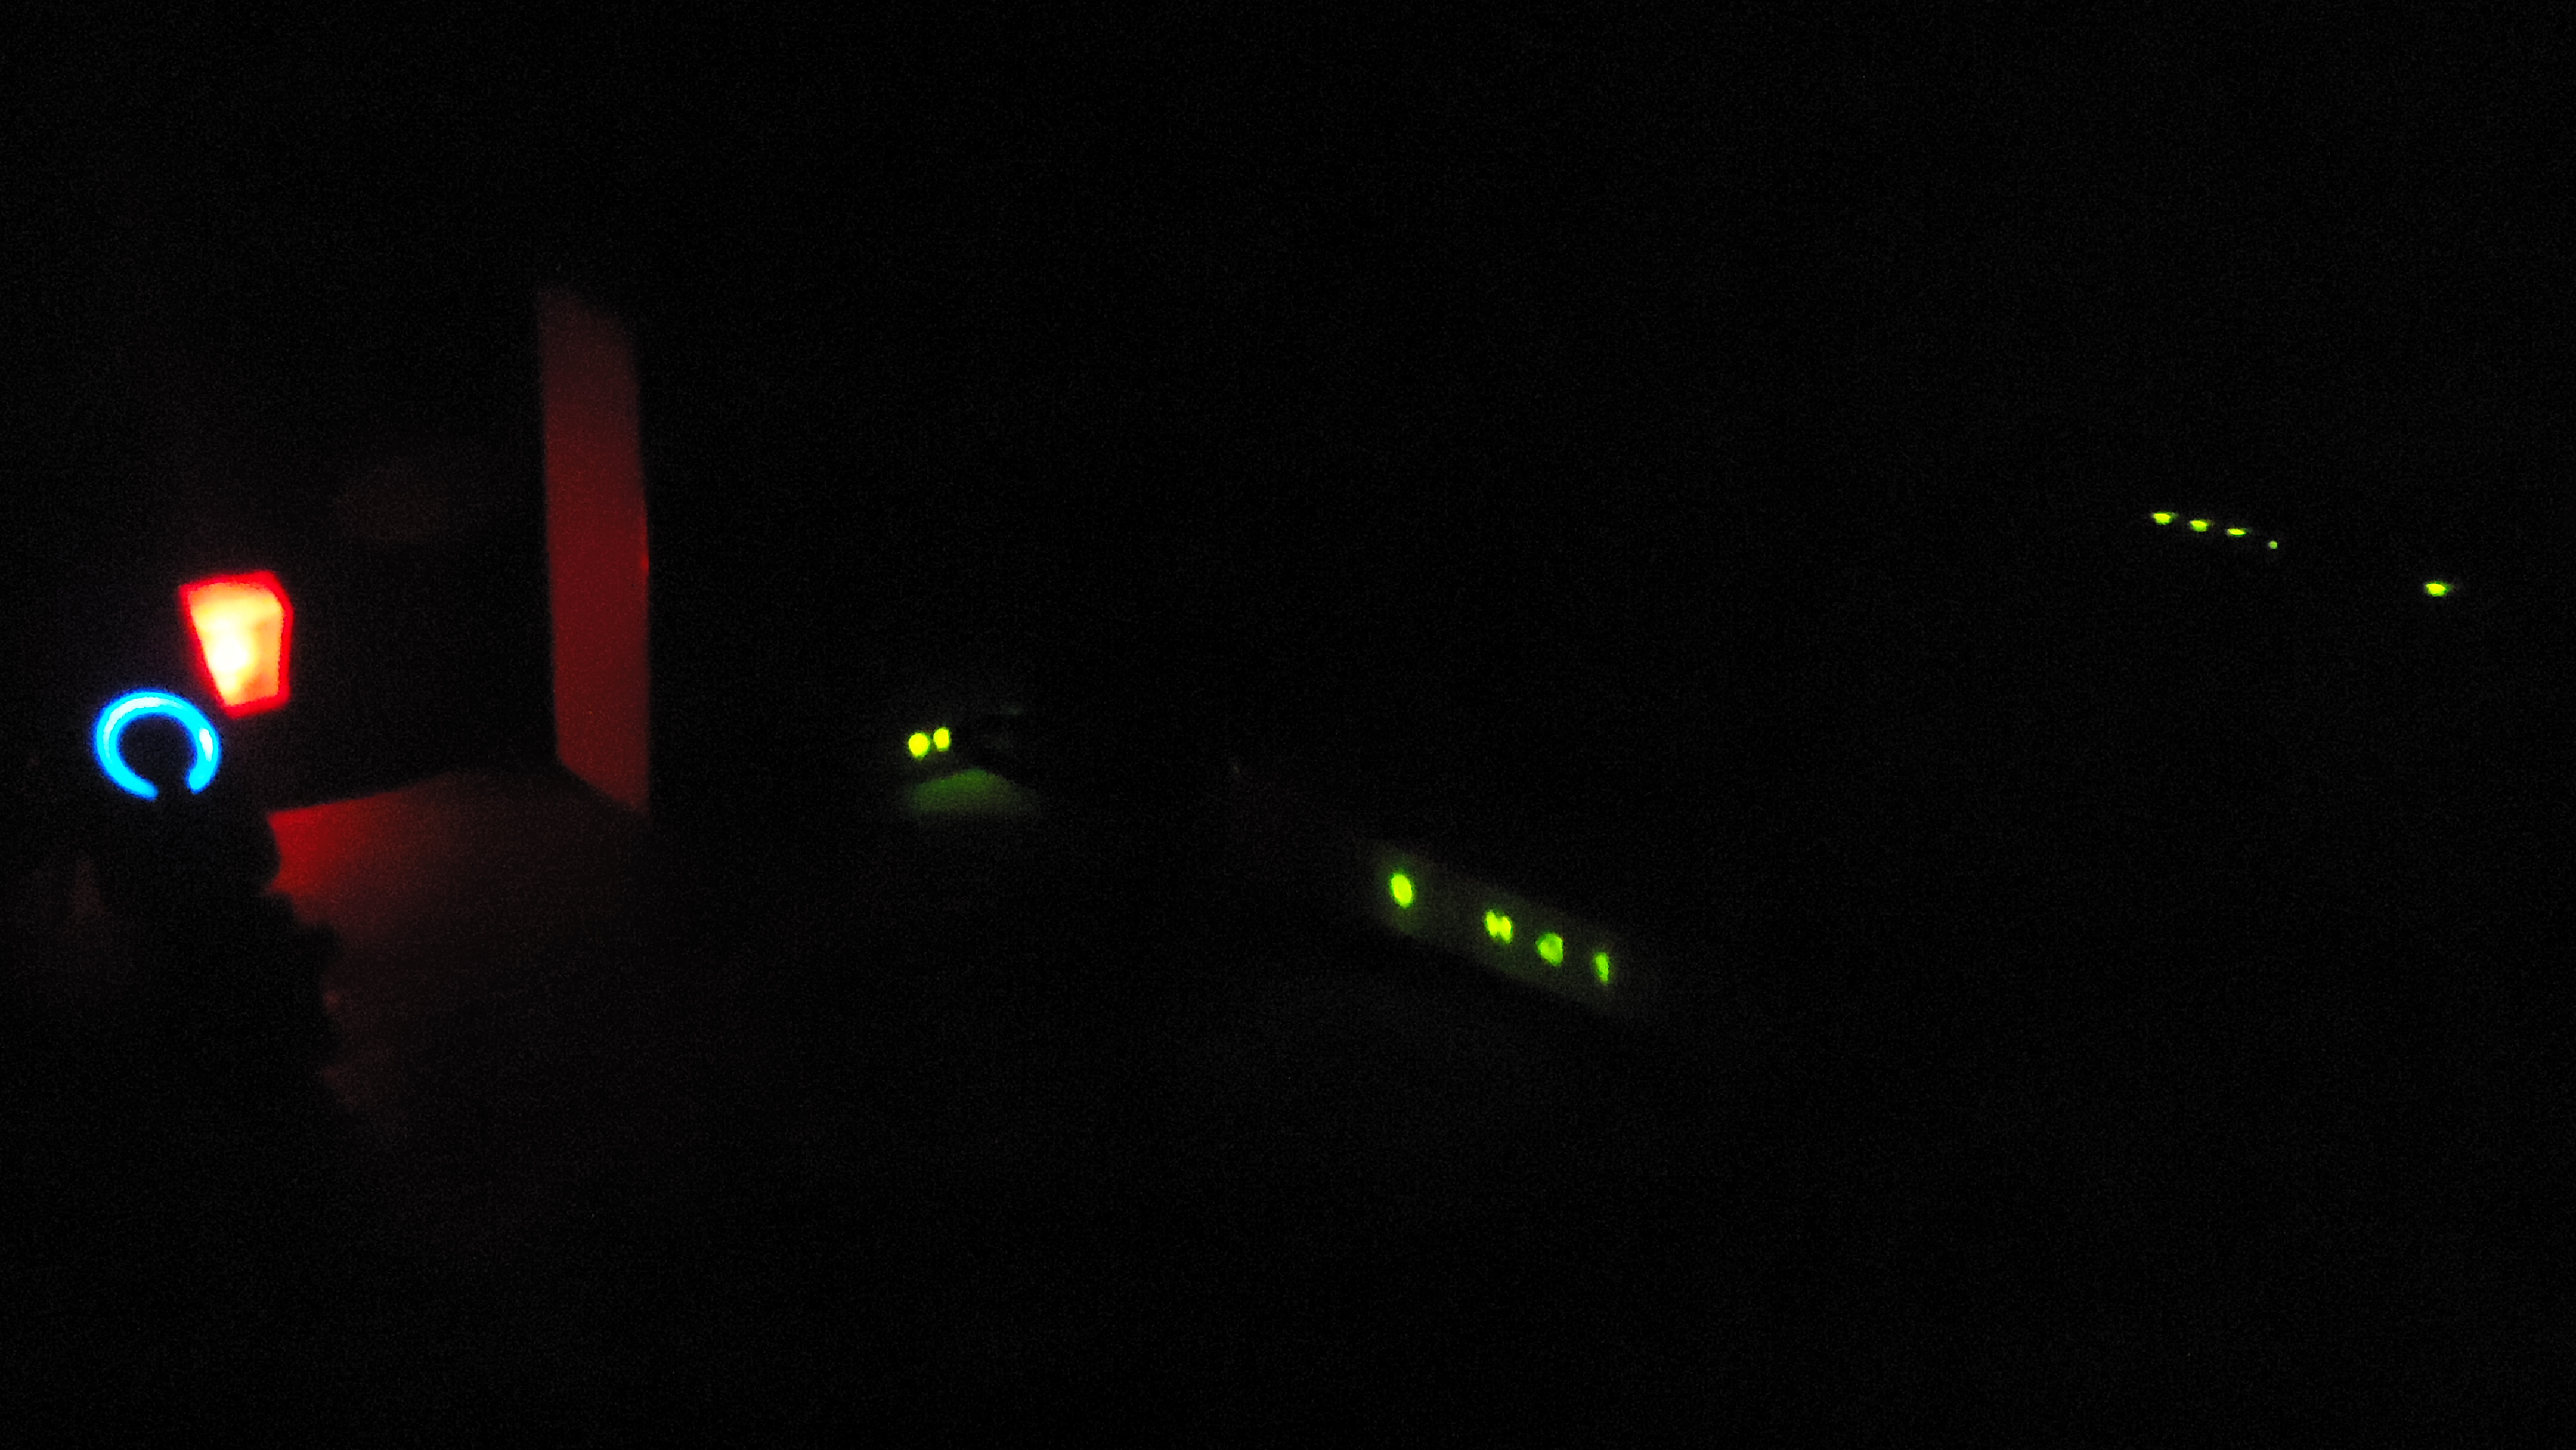
\includegraphics[scale=0.04]{./figures/led.JPG}    
    \caption{LED glowing in the night}   
    \label{fig:led}
   
\end{figure}

\section{Case Studies}
In this section we present some case studies from the data collected in this deployment.
\subsection{Correlating Events}
In this section we show how multi-modal data can be used for activity recognition. Following plots show the same.

\subsection{Water-Energy Nexus}
\subsubsection{Water Filter}
In this section we find out the effective cost of 1 litre of water. RO is known to waste a lot of water. From the water meter we observe the amount of water consumed to fill 1 litre of water. We also see the corresponding power draw of the RO. Thus, we can see that water has energy embedded in it.

\subsubsection{Electric Motor}
Another unique aspect of our setting is the use of electric motor to pump water. Figure showing 1 litre events before motor was turned on and figure showing 1 litre events after motor is turned on.
Figure showing power consumption incurred by the use of motor.

\subsubsection{NILM}
In this section we see the scope of NILM. Might not do this section as it will get very tricky to do NILM on Indian dataset due to variety of reasons.

To highlight any thing or add new stuff write like this in red

\redcolor{This is my comment. I would also do ... and put this image and put this table and so on and so forth}

\section{Conclusions and Future Work}


\balance
\bibliographystyle{abbrv}
\bibliography{references}  % sigproc.bib is the name of the Bibliography in this case
\end{document}
